% \documentclass[a4paper,twoside,openright]{report}
\documentclass[landscape,a4paper]{report}
\usepackage[landscape,driver=xetex,a4paper,margin=25mm]{geometry} % propper margins on a4 paper

\usepackage[hidelinks]{hyperref} % make contents and references clickable in pdf
\usepackage[english]{babel}
\usepackage{fancyhdr}
\usepackage{emptypage}
\usepackage{amsmath}

\usepackage{pstricks-add}
%% \usepackage[official]{eurosym}
\usepackage[nottoc,numbib]{tocbibind}

\usepackage{appendix}

\usepackage{graphicx}
\usepackage{caption}
\graphicspath{{./plaatjes/}}
\DeclareGraphicsExtensions{.png}

% used for typeproofs
\usepackage{amsfonts}
\usepackage{amssymb}
\usepackage{bussproofs}

\usepackage[utf8]{inputenc}

% font stuff
\usepackage{fontspec}
\setmainfont[
   BoldFont={Source Sans Pro Black},
   AutoFakeSlant=0.3
]{Source Serif Pro}
\setmonofont{Source Code Pro}

\usepackage{url}
\usepackage{multicol}
\usepackage[section]{placeins}

\usepackage{enumerate}
\usepackage{enumitem}

\usepackage{listings}
\usepackage{amsmath}
\usepackage{xcolor}
\lstset{%
   basicstyle=\footnotesize\ttfamily,
   frame=single,
   breaklines=true,
   postbreak=\raisebox{0ex}[0ex][0ex]{\ensuremath{\color{red}\hookrightarrow\space}},
   keepspaces=true
}

% draft marker
\usepackage{draftwatermark}

\newcommand*\writer{Louis van der Burg}
% \renewcommand{\chaptermark}[1]{%
% \markboth{#1}{}}

%header & footer
\pagestyle{fancy}
\fancyhf{}
\fancyhead[LE,RO]{\nouppercase\leftmark}
\fancyhead[RE,LO]{\partname\ \thepart}
\fancyfoot[CE,CO]{\writer}
\fancyfoot[LE,RO]{\thepage}

%title page stuff
\fancypagestyle{plain}{%
   \fancyhf{}\fancyfoot[LE,RO]{\thepage}%
   \fancyfoot[CE,CO]{\writer}
\renewcommand{\headrulewidth}{0pt}}

\newcommand\BrText[2]{%
   \par\smallskip
   \noindent\makebox[\textwidth][r]{$\text{#1}\left\{
      \begin{minipage}{\textwidth}
         \lstset{#2}
      \end{minipage}
      \right.\nulldelimiterspace=0pt$}\par\smallskip
   }


\begin{document}

\title{Debugging and expanding Meta Casanova}
\author{\writer}

\begin{titlepage}
   %%%%%%%%%%%%%%%%%%%%%%%%%%%%%%%%%%%%%%%%%
% Formal Text-Rich Title Page
% LaTeX Template
% Version 1.0 (27/12/12)
%
% This template has been downloaded from:
% http://www.LaTeXTemplates.com
%
% Original author:
% Peter Wilson (herries.press@earthlink.net)
%
% License:
% CC BY-NC-SA 3.0 (http://creativecommons.org/licenses/by-nc-sa/3.0/)
%
% Instructions for using this template:
% This title page compiles as is. If you wish to include this title page in
% another document, you will need to copy everything before
% \begin{document} into the preamble of your document. The title page is
% then included using \titleGP within your document.
%
%%%%%%%%%%%%%%%%%%%%%%%%%%%%%%%%%%%%%%%%%

%----------------------------------------------------------------------------------------
%	PACKAGES AND OTHER DOCUMENT CONFIGURATIONS
%----------------------------------------------------------------------------------------

%\documentclass{book}

\newcommand*{\plogo}{\fbox{$\mathcal{PL}$}} % Generic publisher logo

%----------------------------------------------------------------------------------------
%	TITLE PAGE
%----------------------------------------------------------------------------------------

\newcommand*{\titleGP}{\begingroup % Create the command for including the title page in the document
\centering % Center all text
\vspace*{\baselineskip} % White space at the top of the page

\rule{\textwidth}{1.6pt}\vspace*{-\baselineskip}\vspace*{2pt} % Thick horizontal line
\rule{\textwidth}{0.4pt}\\[0.5\baselineskip] % Thin horizontal line

{\LARGE Debugging and expanding \\ [0.4\baselineskip] Meta-Casanova }\\[0.2\baselineskip] % Title

\rule{\textwidth}{0.4pt}\vspace*{-\baselineskip}\vspace{3.2pt} % Thin horizontal line
\rule{\textwidth}{1.6pt}\\[\baselineskip] % Thick horizontal line

\scshape % Small caps
Mandaat\\[\baselineskip] % Tagline(s) or further description
Rotterdam, 2016\par % Location and year

\vspace*{3\baselineskip} % Whitespace between location/year and editors

Written by \\[0.3\baselineskip]
{\Large LOUIS VAN DER BURG \par} % Editor list
{\small 0806963 } \\[0.3\baselineskip] % Editor list
{\itshape Creating 010 \\ Rotterdam\par} % Editor affiliation

\vspace*{1.5\baselineskip} % Whitespace between location/year and editors

\vfill % Whitespace between editor names and publisher logo

%\plogo \\[0.3\baselineskip] % Publisher logo
{\scshape \today} \\[0.3\baselineskip] % Publisher logo
{\scshape versie 1.9} \\[0.3\baselineskip] % Year published

\endgroup}

%----------------------------------------------------------------------------------------
%	BLANK DOCUMENT
%----------------------------------------------------------------------------------------

%\begin{document}

%\pagestyle{empty} % Removes page numbers

\titleGP % This command includes the title page

%\end{document}

\end{titlepage}

\begin{abstract}
   \emph{Debugging and expanding Meta Casanova.}
   The internship will consist of checking the current state of Meta Casanova and improving the syntax and standard library for the user.
   The goal of the assignment is to improve and expand MC.
   The current version of Meta Casanova is still in development and needs to be checked for bugs and faults.
   The usability also needs testing because we want to know how good of a programming language Meta Casanova is.
   The central research question is: \emph{How can the programming language Meta Casanova be improved for the user within the timeframe of the internship?}
   This internship will be executed within the language design field of computer science.
   The internship will be carried out at \emph{Kenniscentrum Creating 010}.
   The research will be qualitative and will make use of descriptive and testing research methods.
   The intended result will consist of a correct and coherent syntax of Meta Casanova together with an implementation of basic programming constructs and higher order type constructs within the standard library.
   The end result will consist of these implementations together with the documentation in the form of a bachelor thesis.
\end{abstract}

\section{Introduction}
\subsection{Working title}
Debugging and expanding Meta Casanova.

\subsection{Motive}
Video game development is difficult~\cite{blow2004game}.
Video games are getting bigger and, with it, more complex.
However the time between releases of the video games does not lengthen~\cite{blow2004game}.

One of the major challenges video game developers face is a short time to market.
When the developers are able to produce games faster, they have an advantage over their competitors.

This is where \emph{Casanova} comes in.
\emph{Casanova} is a programming language to make the development of games easier~\cite{maggiore2011designing}.

Casanova uses higher order types to make the programming of complex constructs easier.
These constructs are often used in game development.

Because of the higher order types the compiler for Casanova became complex.
The compiler for Casanova worked, but was still in development.
So when a bug was found in the compiler, fixing it became more and more time consuming.
This frustrated the developers so much a new language was created~\cite{giuseppe2015mc}.

Meta Casanova (from now on called \emph{MC}) is this new language.
MC serves as the language in which Casanova will be written as a library

At the beginning of the assignment MC was still in development.
The syntax was nearly complete, but untested, and the standard library of MC was just beginning to take shape.
The assignment was created to debug and expand MC and further refine the standard library of MC.


\subsection{Importance}
The result of this thesis will contribute to the development of MC.
The thesis will also serve as documentation for future developers of MC.

\subsection{Goal}\label{sec:goalsmandate}
The goal of the assignment is to debug and expand MC and further refine the standard library within the time limit of the internship.

\subsection{Problem statement}
Currently there are several working versions of MC available, mark I and II, but none of these implement the higher order types.
We want to have a version of MC which contains higher order types.

The newest development version is the one that will be used for this assignment.
The newest version of MC has no working compiler yet and is therefor easily adapted to bugs found during testing.
The newest version of MC also implements new features not present in the previous versions.
Because the newest version of MC is still in development we want to detect any flaws and mishaps in the design during this phase.
This makes otherwise fatal flaws fixable.

The usability of the newest version is also not tested yet and we want to see how good of a programming language MC is for the user.

\subsection{Central research question and sub-questions}
From this problem statement follows the following research question:

\emph{How can the programming language Meta Casanova be improved for the user within the timeframe of the internship?}

The user is a programmer using the language to create applications.

This research question is quite broad and several sub-questions have been created to define a scope for the assignment.

\begin{enumerate}[noitemsep]
   \item What is a good programming language to the user?
   \item What is MC and how does it work?
   \item How can the current syntax be improved to serve the user?
   \item How can the standard library be improved to serve the user?
\end{enumerate}

This also translates to the actual assignment and goal as described in subsection \ref{sec:goalsmandate}.

\subsection{The client}\label{sec:clientmandate}
The graduation assignment will be carried out at Kenniscentrum Creating 010 with the research group of MC.
The company is located in Rotterdam.
\textit{Kenniscentrum Creating 010 is a transdisciplinary design-inclusive Research Center enabling citizens, students and creative industry making the future of Rotterdam}~\cite{creating2016home}.

The research group is active within the language design area of computer sciences.


\subsection{Working environment and tasks}\label{sec:workenvmandate}
During the internship the student will work as a part of the existing research team, who do research in the Casanova and MC languages.
The student will be doing research into programming languages and MC and will program in MC.

The competence \emph{administering} will be attained by further developing MC according to the specifications of the research group.

The competence \emph{Analysing} will be attained by refining the standard library of MC in accordance with what is needed for the user and the research group.

The competence \emph{Advising} will be attained when putting forth improvements for MC.

The competence \emph{Designing} will be attained when debugging MC and refining the standard library to further improve the language.

The student will be supported and helped by the entire research team.
Every two weeks the student will present his progress and receive feedback from the research group.


\section{Method}\label{ch:methodmandate}
\subsection{Research methods}
During the internship there will be made use of different research methods.
This stems from the wide scope of the project and the fact that there are multiple research questions which require different approaches.

We will now describe what the research methods per sub-question are.


\subsubsection{What is a good programming language to the user?}
This question will be answered by describing what a good programming language is to the user.
The results of this description will then be compared to MC and where necessary implemented in to MC without compromising the ideas and philosophies behind MC.

\subsubsection{What is MC and how does it work?}
This question will be answered by describing the ideas and philosophies behind MC.
To further grasp what MC is, the syntax will be described and the standard library explained.

\subsubsection{How can the current syntax be improved to serve the user?}
This question will be answered by comparing the existing syntax to the ideas and philosophies of MC.
The syntax will also be tested for correctness and coherence.

\textbf{MC will be futher tested by creating test programs.... DO THIS MAYBE?????}
test programs are written to test the syntax of the language.

\subsubsection{How can the standard library be improved and refined to serve the user?}
This question will be answered by describing the standard library and implementing constructs often used in programming.
Constructs using higher order types will also be implemented after describing what they are and what they do.



\subsection{Gathering information}
The information that is needed to answer the research questions are stated in the questions themselves.


\subsubsection{What is a good programming language to the user?}
There is no quality standard predefined for what a good programming language is.
Therefor the information for this question will be gathered from research papers, specifically those who are based on interviews with experienced users or are written by experienced users.

\subsubsection{What is MC and how does it work?}
The information for this question will be gathered from the research group and the papers written by them.
This will be done by interviewing the research group.

\subsubsection{How can the current syntax be improved to serve the user?}
The information for this question will be gathered by having a description of both MC and what makes a programming language good to the user.
These descriptions will be gathered by answering the previous two research questions.

\subsubsection{How can the standard library be improved and refined to serve the user?}
The information for this question will be gathered by describing the standard library and holding interviews with the research group.
The interviews will result what is absolutely needed in the standard library.


\subsection{Validation of results}
The validity of the results will be secured by regularly discussing with the client and the supervisor.
All the improvements and expansions added to MC and the standard library will be double checked and discussed with the research group to prevent any inconsistencies from occurring.


\subsection{Validity and trustworthiness of sources}
The sources used will be published papers and personal interviews with the research group.
The papers must be relative to the subject matter.

All the sources used need to be approved by the research group and the supervisor.


\subsection{Project methods}
During the internship the LEAN-software development method will be used\cite{ries2011lean}.

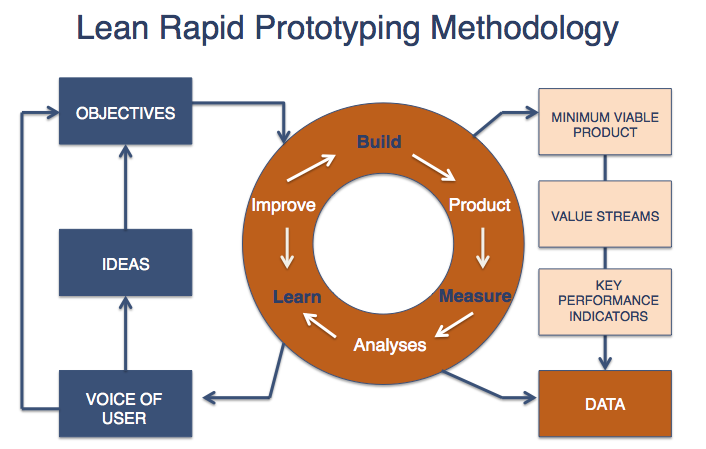
\includegraphics[width=\textwidth]{lean}

Using LEAN gives the ability to quickly iterate through versions and gather knowledge more easily through these iterations.

When using LEAN results are fast available.
These results can be used to catch faults early on and adjust the project accordingly.


\subsection{Risk analyses}
\begin{center}
   \begin{tabular}
      {| p{0.2\textwidth} | p{0.25\textwidth} | l | p{0.3\textwidth} |}
      \hline
      \textbf{Risk} & \textbf{Effect} & \textbf{Possibility} & \textbf{Counter measure}
      \\ \hline
      Quick development of the language. & Because the language becomes bigger as time progresses, the assignment could become too large to do in the set time. & 70\% & The analyses and development of MC will take place for a limited period of time, which prevents the project going on for too long.
      \\ \hline
      The compiler is not finished at the time. & MC can not be tested in practice. & 80\% & The code will be manually checked for errors by the student and the research group.
      \\ \hline
      The supervisor falls ill for a prolonged period. & The student has no direct contact point for questions and might get stuck. & 15\% & The student is introduced to the entire research group so he can ask or contact them as well for questions.
      \\ \hline
      The company goes bankrupt during the internship. & The assignment will not be finished and the student will not be able to graduate. & 1\% & There is nothing the student can do to prevent this.
      \\ \hline
   \end{tabular}
\end{center}

\subsection{Quality expectations}
MC makes use of type theory and the programs written in it will therefor need to be in line with the type theory, as described in \emph{Types and programming languages}~\cite{pierce2002types}.
Because the version of MC used in this internship has no compiler yet, the student will need to manually make sure that the syntax and standard library have no bugs and/or errors in them.

\section{Results}
\subsection{Intended result}
The end result should be a correct and coherent syntax for MC.
Adding to this the standard library should have at least a few basic programming constructs and higher order type constructs.


\bibliographystyle{ieeetr}
\bibliography{biblio}

\begin{appendices}
   \chapter{Stakeholders}
% \renewcommand{\abstractname}{Stakeholders}
% \begin{abstract}
   % \hfill
   % \vfill
   % \columnbreak
\begin{multicols}{2}

   \begin{tabular}
      { l l }
      \textbf{The graduate} & \\
      Name & Louis van der Burg \\
      Student number & 0806963 \\
      E-mail address & louis.burg@hotmail.com \\
      Telephone number & +31 6 14 85 55 79 \\
      & \\
      \textbf{Client} & \\
      Name company & Kennis Centrum Creating 010 \\
      Name company supervisor & Sunil Choenni \\
      E-mail address & h.choenni@hr.nl \\
      Telephone number & +31 6 48 10 03 01  \\
      Function & Lector \\
      Visitors address & Wijnhaven 103 verdieping 6 \\
      Website company & www.creating010.com \\
   % \end{tabular}
   % \begin{tabular}
      % { l l }
      & \\
      \textbf{Company supervisor} & \\
      Name company & Kennis Centrum Creating 010 \\
      Name company supervisor & Sunil Choenni \\
      E-mail address & h.choenni@hr.nl \\
      Telephone number & +31 6 48 10 03 01  \\
      Function & Lector \\
      Visitors address & Wijnhaven 103 verdieping 6 \\
      Website company & www.creating010.com \\
      & \\
      \textbf{School supervisors} & \\
      Name examinator (first teacher) & Giuseppe Magiorre \\
      E-mail address & +31 6 41 78 12 23 \\
      Telephone number & g.maggiore@hr.nl \\
      Name assessor (second teacher) & Hans Manni \\
      E-mail address & j.p.manni@hr.nl \\
      Telephone number & \\
      & \\
      \textbf{School co\"ordinator} & \\
      Name graduate coördinator INF/TI & Aad van Raamt \\
      Telephone number & 010 7944993 \\
      E-mail address & A.van.Raamt@HRO.NL \\
   \end{tabular}
\end{multicols}
% \end{abstract}

\end{appendices}
\end{document}
